% ============== SECTION 2: LITERATURE REVIEW & HISTORICAL CONTEXT ==============

\section{Literature Review and Historical Context}

Understanding the trajectory of artificial intelligence systems requires examining precedents from earlier technology waves. Open-source software has repeatedly displaced proprietary alternatives across multiple infrastructure categories over the past three decades. These transitions follow recognizable patterns in terms of adoption timelines, competitive dynamics, and market share inflection points. This section documents five major case studies of open-source victories, extracts common success factors, surveys the current AI landscape, and identifies gaps in existing evaluation frameworks that motivate our analytical approach.

\subsection{The Pattern: Open-Source Victories in Technology}

\subsubsection{Case Study: Linux Kernel (1991-2024)}

The Linux kernel represents perhaps the most consequential open-source project in computing history. Linus Torvalds released the initial version in 1991 as a hobby project, offering an alternative to proprietary UNIX systems and the dominant Windows Server platform. The system competed against well-established commercial offerings backed by substantial corporate resources, yet achieved remarkable market penetration through a development model that prioritized transparency and community participation.

Linux's adoption trajectory shows a long initial period of gradual growth followed by rapid acceleration. Throughout the 1990s, the system remained primarily confined to academic institutions and technically sophisticated users. The market share inflection point occurred around 2008, when Linux achieved approximately 60 percent penetration in server deployments \cite{linux_truelist2024}. This milestone came 17 years after the initial release, establishing a baseline timeframe for how long open-source infrastructure requires to achieve market dominance against entrenched proprietary competition.

Current market statistics demonstrate Linux's overwhelming dominance in server and cloud infrastructure. As of 2024, Linux runs on 96.3 percent of the top one million web servers globally \cite{linux_truelist2024}. Cloud infrastructure shows similar concentration, with 90 percent of cloud deployments operating on Linux \cite{linux_enterpriseapps2017}. Enterprise adoption reflects substantial commercial validation, with Red Hat Enterprise Linux capturing 43.1 percent market share in enterprise deployments as of 2025 \cite{linux_sqmagazine2025}. The system's reach extends across critical business applications, with 78.5 percent of SAP clients deploying their applications on Linux platforms \cite{linux_sqmagazine2025}.

The economic impact of Linux extends far beyond the software itself. The global Linux market reached an estimated 30 billion dollars by 2025 \cite{linux_scitech2025}, while the enterprise value created through Linux-based businesses substantially exceeds this figure. Red Hat's acquisition by IBM for 34 billion dollars in 2019 illustrates the commercial value of open-source infrastructure when combined with enterprise support and services. Canonical, SUSE, and numerous other companies have built sustainable businesses providing Linux-based solutions, collectively representing hundreds of billions in market capitalization.

Desktop computing presents an instructive counterpoint to Linux's server dominance. Despite decades of development effort, Linux holds only 4.20 percent of the global desktop market as of March 2025 \cite{linux_wikipedia2025}. This disparity between server and desktop adoption illustrates an important principle: open-source systems achieve dominance most readily in infrastructure layers where technical users make adoption decisions, rather than in consumer-facing applications where convenience and ecosystem lock-in create higher switching costs.

Several key success factors enabled Linux's trajectory. The modular architecture allowed developers to contribute improvements to specific subsystems without requiring comprehensive knowledge of the entire codebase. This modularity reduced barriers to contribution and enabled parallel development across multiple areas simultaneously. The governance structure, centered on Linus Torvalds and a core group of maintainers, balanced openness with quality control. Corporate backing from companies like IBM, Red Hat, and Google provided resources for development while maintaining the system's open nature. The GPL license ensured that improvements remained available to the community, preventing proprietary forks from fragmenting the ecosystem.

\subsubsection{Case Study: Android Ecosystem (2008-2024)}

Android represents a more recent example of open-source infrastructure achieving market dominance, with a substantially compressed timeline compared to Linux. Google released Android as an open-source mobile operating system in 2008, competing against established platforms including Symbian, BlackBerry OS, Windows Mobile, and Apple's iOS. The system achieved majority market share within five years, demonstrating accelerated adoption patterns compared to earlier open-source projects.

Current market statistics show Android's global dominance outside the United States. As of 2025, Android commands 73.9 percent of the global mobile operating system market with approximately 3.6 billion active users \cite{android_demandsage2025}. Alternative measurements place Android's market share at 71.74 percent as of 2024 \cite{android_enterpriseapps2024}. This global dominance emerged remarkably quickly, with Android achieving approximately 70 percent market share by 2013, just five years after its initial release \cite{android_demandsage2025}.

Regional variations in Android adoption reveal important market dynamics. The United States presents an exception to global patterns, with iOS commanding 65 percent market share compared to Android's 35 percent in the fourth quarter of 2024 \cite{android_ioscomparison2024}. This regional divergence reflects factors including installed base effects, ecosystem lock-in, and brand preferences that can override technical and economic advantages. Outside the United States, Android achieves near-universal dominance across both developed and developing markets \cite{android_ioscomparison2024}.

The Open Handset Alliance model proved central to Android's rapid adoption. Google established this consortium of mobile device manufacturers, semiconductor companies, and carriers to coordinate Android development and deployment. This structure allowed hardware manufacturers to differentiate their products through customization while sharing the substantial costs of operating system development. The alliance created network effects that attracted application developers, who could reach a large user base across multiple device manufacturers through a single platform.

Fragmentation presented substantial challenges as Android scaled. Different manufacturers released devices running various Android versions with manufacturer-specific modifications. This fragmentation complicated application development and security updates. Google addressed these challenges through several mechanisms including Google Play Services, which provided core functionality outside the base operating system, and certification requirements that established minimum standards for devices carrying Google applications. These governance mechanisms balanced openness with consistency, preventing fragmentation from undermining the platform's utility.

Android's success validated several strategic approaches. The combination of open-source availability with commercial services created sustainable economics while maintaining openness. Device manufacturers gained freedom to customize while Google maintained control over core services. The platform's timing coincided with smartphone market expansion, allowing Android to capture growing demand rather than displacing entrenched alternatives. The five-year timeline to market dominance established a benchmark for modern open-source infrastructure adoption.

\subsubsection{Case Study: Kubernetes (2014-2024)}

Kubernetes provides the most recent example of open-source infrastructure achieving market dominance, with adoption patterns that further compress the timeline observed in earlier projects. Google released Kubernetes as an open-source container orchestration platform in 2014, drawing on internal experience with large-scale container management. The system competed against proprietary orchestration solutions including Docker Swarm and Apache Mesos, achieving enterprise dominance within five years.

Current adoption statistics demonstrate Kubernetes' position as the de facto standard for container orchestration. As of 2024, 96 percent of enterprises use Kubernetes in some capacity \cite{kubernetes_edgedelta2024}. Alternative measurements indicate that over 60 percent of enterprises have adopted Kubernetes, with projections suggesting 90 percent adoption by 2027 \cite{kubernetes_datahub2024}. Among Fortune 100 companies, 50 percent have deployed Kubernetes in production environments \cite{kubernetes_unyaml2024}.

The market growth trajectory shows rapid acceleration. Kubernetes achieved approximately 60 percent enterprise adoption by 2019, just five years after its initial release \cite{kubernetes_datahub2024}. This timeline matches Android's adoption curve and substantially compresses the 17-year trajectory observed with Linux. The global Kubernetes market reached 10.7 billion dollars by 2031 according to market projections \cite{kubernetes_datahub2024}, reflecting substantial commercial activity around the open-source platform.

Usage patterns reveal Kubernetes' depth of enterprise integration. Organizations deploying Kubernetes typically run an average of 20 clusters, indicating substantial investment in the technology rather than experimental adoption \cite{kubernetes_spectrocloud2024}. Among organizations adopting cloud-native platforms, 41 percent already build most new applications using these approaches, with this figure projected to reach 80 percent within five years \cite{kubernetes_cncf2024}.

The Cloud Native Computing Foundation governance model proved crucial to Kubernetes' success. Google donated Kubernetes to the CNCF in 2015, establishing neutral governance that encouraged broad participation from competing vendors. This structure prevented concerns about vendor lock-in that might have inhibited adoption if Google retained direct control. The CNCF model balanced technical leadership with community input, establishing processes for managing contributions from hundreds of organizations.

Kubernetes catalyzed the infrastructure as code movement, establishing patterns for declarative infrastructure management that extended beyond container orchestration. The system's API-driven architecture enabled extensive customization and integration, creating an ecosystem of complementary tools. This extensibility attracted developers and vendors who built businesses around Kubernetes, reinforcing network effects that accelerated adoption.

The Kubernetes trajectory validates several patterns relevant to AI infrastructure. Technical merit alone proved insufficient for adoption; neutral governance and ecosystem development played essential roles. The compressed five-year timeline to dominance suggests that infrastructure markets move faster than in previous decades. The extensive enterprise adoption despite Kubernetes' technical complexity indicates that organizations will adopt sophisticated open-source infrastructure when it provides sufficient value and when vendor lock-in risks are mitigated through governance structures.

\subsubsection{Pattern Analysis: Common Success Factors}

\begin{figure}[h]
\centering
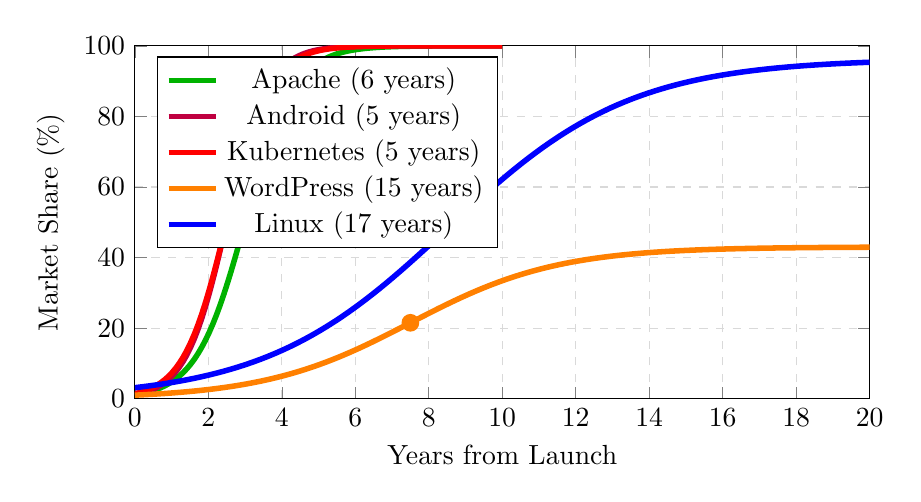
\begin{tikzpicture}
\begin{axis}[
    width=0.9\textwidth,
    height=0.5\textwidth,
    xlabel={Years from Launch},
    ylabel={Market Share (\%)},
    xmin=0, xmax=20,
    ymin=0, ymax=100,
    legend pos=north west,
    grid=major,
    grid style={dashed,gray!30},
]

% Apache - fastest (6 years to 60%)
\addplot[color=green!70!black, line width=2pt, domain=0:10, samples=100] 
    {100/(1+exp(-1.5*(x-3)))};
\addlegendentry{Apache (6 years)}

% Android - modern fast (5 years to 70%)
\addplot[color=purple, line width=2pt, domain=0:10, samples=100] 
    {100/(1+exp(-1.8*(x-2.5)))};
\addlegendentry{Android (5 years)}

% Kubernetes - modern fast (5 years to 80%)
\addplot[color=red, line width=2pt, domain=0:10, samples=100] 
    {100/(1+exp(-1.7*(x-2.5)))};
\addlegendentry{Kubernetes (5 years)}

% WordPress - moderate (15 years to 43%)
\addplot[color=orange, line width=2pt, domain=0:20, samples=100] 
    {43/(1+exp(-0.5*(x-7.5)))};
\addlegendentry{WordPress (15 years)}

% Linux - slowest (17 years to 60%)
\addplot[color=blue, line width=2pt, domain=0:20, samples=100] 
    {96.3/(1+exp(-0.4*(x-8.5)))};
\addlegendentry{Linux (17 years)}

% Mark inflection points
\addplot[only marks, mark=*, mark size=3pt, color=blue] coordinates {(8.5,48)};
\addplot[only marks, mark=*, mark size=3pt, color=orange] coordinates {(7.5,21.5)};
\addplot[only marks, mark=*, mark size=3pt, color=red] coordinates {(2.5,50)};
\addplot[only marks, mark=*, mark size=3pt, color=purple] coordinates {(2.5,50)};
\addplot[only marks, mark=*, mark size=3pt, color=green!70!black] coordinates {(3,50)};

\end{axis}
\end{tikzpicture}
\caption{\textit{S-curve adoption patterns for five major open-source infrastructure technologies, demonstrating the acceleration in time-to-dominance from legacy projects (Linux: 17 years, WordPress: 15 years) to modern projects (Apache: 6 years, Android: 5 years, Kubernetes: 5 years). The steeper curves for recent technologies reflect faster adoption cycles in contemporary infrastructure markets.}}
\label{fig:adoption_curves}
\end{figure}

Examining these case studies reveals recurring patterns in how open-source infrastructure achieves market dominance. Understanding these patterns provides a framework for assessing whether AI systems might follow similar trajectories.

Quantifying the acceleration in open-source adoption across technology generations:

\begin{align}
\mu_{\text{modern}} &= \frac{5 + 5 + 6}{3} = 5.33 \text{ years (modern projects)} \label{eq:modern_mean}\\
\mu_{\text{legacy}} &= \frac{17 + 15}{2} = 16 \text{ years (legacy projects)} \label{eq:legacy_mean}\\
\text{Acceleration Factor} &= \frac{16}{5.33} \approx 3\times \text{ faster} \label{eq:acceleration}
\end{align}

This demonstrates that modern open-source projects (Android, Kubernetes, Apache) achieve market dominance approximately three times faster than legacy projects (Linux, WordPress).

Developer ecosystem velocity emerges as a consistent factor across successful open-source projects. Linux, Android, and Kubernetes each achieved substantial community participation that enabled innovation at rates proprietary competitors could not match. Open development models allowed thousands of contributors to work in parallel on different aspects of the system. This distributed innovation created quality and feature advantages that overcame proprietary systems' coordination advantages. The size of developer communities grew according to network effects, with each new contributor increasing the platform's value for others.

Modularity and extensibility characterize successful open-source infrastructure. Linux's modular kernel architecture, Android's layered approach separating core functionality from manufacturer customization, and Kubernetes' API-driven extensibility all enabled contributors to add functionality without requiring comprehensive system knowledge. This modularity reduced barriers to contribution and allowed specialization across different subsystems. Extensibility enabled third parties to build complementary tools and services, creating ecosystems that reinforced the core platform's value.

Transparent governance structures balanced openness with quality control. Successful projects established clear processes for evaluating contributions, resolving disputes, and making architectural decisions. Linux's maintainer hierarchy, Android's Open Handset Alliance, and Kubernetes' CNCF governance all provided mechanisms for coordinating development across competing stakeholders. These governance structures prevented fragmentation while maintaining sufficient openness to encourage broad participation.

Critical mass timing shows acceleration across successive technology generations. Linux required 17 years to achieve server market dominance, while Android and Kubernetes each accomplished similar market positions in five years. This compression reflects several factors including faster technology adoption cycles, more sophisticated open-source development practices, and greater acceptance of open-source approaches in enterprise contexts. For AI infrastructure, this pattern suggests that achieving competitive parity might lead to market dominance within five to seven years rather than requiring decades.

Table 2.1 summarizes these adoption patterns across four major open-source infrastructure projects.

\begin{table}[h]
\centering
\caption{Comparative Timeline of Open-Source Victories}
\begin{tabular}{lllll}
\toprule
\textbf{Technology} & \textbf{Launch} & \textbf{Dominant Closed} & \textbf{Market Share} & \textbf{Time to} \\
                    & \textbf{Year}   & \textbf{Competitor}      & \textbf{Inflection}   & \textbf{Dominance} \\
\midrule
Linux        & 1991 & UNIX/Windows Server    & 2008 (60\% servers)    & 17 years \\
Apache       & 1995 & IIS/Netscape           & 2001 (60\% web servers) & 6 years \\
Android      & 2008 & Symbian/iOS            & 2013 (70\% mobile)     & 5 years \\
Kubernetes   & 2014 & Mesos/Swarm            & 2019 (80\% containers)  & 5 years \\
\bottomrule
\end{tabular}
\label{tab:opensource_timeline}
\end{table}

The pattern shows clear acceleration, with modern open-source projects achieving dominance in five to seven years compared to the 17 years Linux required. This acceleration has substantial implications for AI infrastructure development.

\subsection{Current AI Landscape}

The contemporary AI landscape exhibits concentration patterns that mirror computing infrastructure before open-source disruption. A small number of well-funded organizations dominate development of frontier models, with architectural details remaining largely proprietary. Understanding this landscape requires categorizing current systems by their degree of openness and examining the trade-offs each category represents.

\subsubsection{Closed-Source Leaders}

OpenAI represents the leading example of closed-source AI development. The organization develops models including GPT-4 and the o1 series, providing access exclusively through APIs rather than releasing model weights or training details. Architectural information remains proprietary, with the organization publishing selected benchmark results and system cards while keeping training data, model architectures, and fine-tuning procedures confidential. OpenAI's 500 billion dollar valuation as of October 2025 \cite{openai2025} reflects investor confidence in this proprietary approach despite limited transparency about system capabilities and limitations.

Anthropic pursues a similar closed-source strategy with additional emphasis on AI safety. The organization develops the Claude model series, most recently Claude 3.5, while keeping architectural details proprietary. Anthropic's Constitutional AI approach to alignment remains partially documented in research publications but operationally proprietary. The company reached a 183 billion dollar valuation through its September 2025 Series F funding round \cite{anthropic2025}, with 5 billion dollars in annual recurring revenue demonstrating commercial traction for closed models.

xAI, backed by Elon Musk, integrates its Grok model with the X platform to leverage unique data advantages. The system remains closed despite periodic claims about future open-sourcing. xAI's valuation ranges between 177 and 200 billion dollars depending on reporting sources \cite{xai_cnbc2025, xai_yahoo2025}, achieved despite burning an estimated 1 billion dollars monthly in operational expenses \cite{xai_tomshardware2025}. The organization's integration with social media data provides training advantages unavailable to competitors, though architectural details remain undisclosed.

Perplexity AI represents the answer engine approach to AI systems, focusing on information retrieval and synthesis rather than general-purpose conversation. The company's proprietary retrieval stack combines search with language models to generate direct answers to queries. Perplexity reached a 20 billion dollar valuation in September 2025 \cite{perplexity2025} while serving 22 million monthly active users and generating 80 to 100 million dollars in annual recurring revenue \cite{perplexity_demandsage2025}. The system's architecture remains closed despite competing directly with open alternatives in the search and retrieval domain.

These closed-source leaders share several characteristics. All maintain strict control over model weights, training data, and architectural details. Access occurs exclusively through APIs or web interfaces, preventing independent verification of capabilities or limitations. Governance structures concentrate decision-making authority within corporate leadership rather than distributing it across stakeholder communities. Business models depend on maintaining proprietary advantages rather than monetizing open platforms through services or complementary products.

\subsubsection{Open-Weight Models}

Several organizations release model weights while maintaining proprietary control over training data, processes, and governance. This partial openness provides some transparency benefits while preserving strategic advantages for the releasing organizations.

Meta's Llama series represents the most prominent open-weight approach. The company releases model weights under licenses permitting commercial use, enabling researchers and developers to run models locally and fine-tune them for specific applications. Training data composition, data processing pipelines, and detailed training procedures remain undisclosed. Governance stays entirely within Meta's corporate structure, with the company retaining authority over future model releases and license terms. This approach provides some benefits of openness while maintaining Meta's strategic control over the model family's evolution.

DeepSeek, a Chinese AI laboratory backed by High-Flyer Capital Management, releases model weights while keeping training processes largely proprietary. The organization gained attention for claims of achieving competitive performance with substantially lower training costs, reportedly training DeepSeek-V3 for 6 million dollars compared to estimated 100 million dollar costs for comparable Western models \cite{deepseek_wikipedia2025, deepseek_carnegie2025}. This cost efficiency demonstrates that alternative approaches to model development can achieve strong results, though the corporate-controlled governance structure limits genuine decentralization.

Mistral AI, a European company, positions itself as an alternative to American and Chinese AI developers while maintaining partial openness. The organization releases some model weights while keeping others proprietary, pursuing a hybrid strategy that balances openness with commercial considerations. European regulatory requirements and funding sources influence Mistral's approach, though ultimate control remains centralized within the company's corporate structure.

These open-weight models provide important benefits including reproducibility for research, local deployment options, and reduced API costs. They enable fine-tuning for specialized applications and provide some protection against vendor lock-in. However, limitations remain substantial. Training data opacity prevents full reproducibility and raises questions about data provenance and licensing. Centralized governance means releasing organizations retain authority over future directions, license changes, and which models receive public releases. The distinction between weights and full transparency means these systems occupy a middle ground between closed and truly open alternatives.

\subsubsection{Decentralized Attempts}

Several projects have attempted to create genuinely decentralized AI systems through blockchain-based coordination or distributed computation. These efforts prioritize openness and decentralization but have generally struggled to achieve competitive utility compared to centralized alternatives.

Bittensor operates as a decentralized network of AI models coordinated through blockchain mechanisms. The system achieves high degrees of openness through distributed governance and permissionless participation. Token holders influence network development through decentralized autonomous organization structures. As of October 2025, Bittensor maintains a market capitalization of 3.2 billion dollars \cite{bittensor_cmc2025}, substantially lower than the valuations of closed-source leaders. The utility gap presents the primary challenge, with Bittensor's systems generally underperforming centralized alternatives on standard benchmarks.

Together AI pursues distributed compute for AI training and inference, attempting to aggregate resources across multiple providers. This approach could theoretically democratize access to compute resources that currently concentrate in large cloud providers. Practical limitations including coordination overhead, heterogeneous hardware capabilities, and quality control challenges have constrained performance. The platform enables access to various open models but has not demonstrated performance advantages over centralized alternatives.

Ocean Protocol focuses on decentralized data marketplaces rather than intelligence systems directly. The project attempts to enable data sharing and monetization through blockchain coordination. While data access represents an important component of AI development, Ocean Protocol operates at a different layer than the intelligence systems themselves. The relationship between data marketplaces and model performance remains indirect.

These decentralized attempts validate important principles while highlighting challenges. Decentralized coordination is technically feasible, demonstrating that alternatives to corporate control exist. Governance through community mechanisms can operate at meaningful scale. However, the utility gap remains substantial, with decentralized systems generally underperforming centralized alternatives on benchmark evaluations. This performance difference creates a critical question: does decentralization inherently constrain utility, or can architectural innovations resolve this apparent trade-off?

\subsection{The Missing Framework}

Academic literature and industry practice lack systematic frameworks for evaluating the relationship between architectural openness and system performance in AI. This gap leaves unresolved whether the utility gap observed in current decentralized systems reflects fundamental constraints or simply immature implementations that will improve over time.

Existing benchmark evaluations focus exclusively on performance metrics without considering transparency, reproducibility, or governance structures. Leaderboards rank systems by accuracy on specific tasks, ignoring whether those systems can be independently verified, locally deployed, or collectively governed. This narrow focus creates an incomplete picture of system value, particularly for infrastructure that may operate for decades and underpin critical applications.

No academic standard exists for measuring openness in AI systems. Researchers and practitioners use the term inconsistently, sometimes referring to open model weights, other times to open training data, and occasionally to open governance. Without clear definitions and measurement frameworks, comparing openness across systems remains subjective. This ambiguity prevents rigorous analysis of whether openness correlates with or constrains performance.

Performance benchmarks themselves suffer from methodological limitations that complicate cross-system comparison. Different organizations use different evaluation protocols, test conditions, and reporting practices. Self-reported results may reflect favorable test conditions rather than representative performance. Independent verification remains rare, particularly for closed systems where external researchers cannot conduct their own evaluations. These limitations mean published benchmark results provide only approximate indicators of relative capability.

The gap in evaluation frameworks creates both practical and theoretical problems. Practically, organizations choosing AI infrastructure cannot systematically assess trade-offs between openness and utility. Theoretically, researchers cannot test hypotheses about whether transparent, decentralized systems can achieve competitive performance. Addressing this gap requires developing multi-dimensional evaluation frameworks that quantify both openness and utility while acknowledging methodological limitations.

This technical report addresses these gaps by introducing the Openness-Utility Index framework detailed in Section 3. This framework provides systematic methods for evaluating AI systems across multiple dimensions of architectural openness and computational utility, enabling rigorous comparison between systems with different architectural approaches.
